\documentclass{article}

\begin{document}


\setlength{\parindent}{6ex}

\begin{figure}
    \centering
    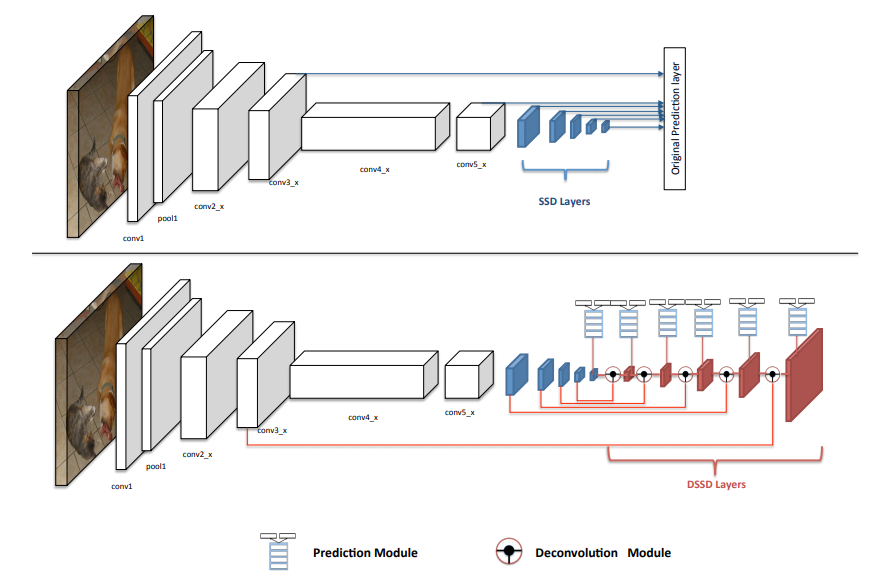
\includegraphics[width=\textwidth]{models/dssd.png}
    \caption{Networks of SSD and DSSD on ResNet}
    \label{fig:dssd1}
\end{figure}

\indent

Deconvolutional Single Shot Detector aims to contribute a new approach for object 
detection. The major changes in DSSD are to change the base network from VGG16 to 
ResNet101, using prediction modules, and adding deconvolution layers after convolutional 
layers of SSD. In figure \ref{fig:dssd1}, you can see the DSSD layers and the way they are 
connected with the layer before and corresponding size SSD layer. Also, the change in 
prediction layer from SSD to DSSD can be seen. So, these changes will be examined as follows: 
\begin{enumerate}
    \item ResNet101
    \begin{itemize}
        \item The aim of changing base network from VGG16 to ResNet101 is to 
increase accuracy. However, it does not improve accuracy by itself. That's why, 
the prediction module is used to increase performance.
    \end{itemize}
    \item Prediction Module
    \begin{itemize}
        \item Due to the principle of improving sub-network can improve accuracy, 
original SSD approach for parameters prediction is replaced with a prediction module which 
consists of a residual block. Thus, using ResNet101 with prediction module performs 
better than VGG16. The implementation of prediction module can be seen in figure 
\ref{fig:predmod1}.
    \end{itemize}
    \item Deconvolution Layers
    \begin{itemize}
        \item The aim of using deconvolutional layers is to include more high-level 
context in detection, so that, deconvolution module integrates information from both 
earlier feature maps and earlier deconvolution layers. Instead of using deconvolution 
module, upsampling layers would have been used to increase the resolution of feature 
maps such as in hourglass networks. However, using deconvolution module provides 
learnable parameters which performs better. You can see the implementation of 
deconvolution module in figure \ref{fig:deconvmod1}.
    \end{itemize}
\end{enumerate}

\begin{figure}
    \centering
    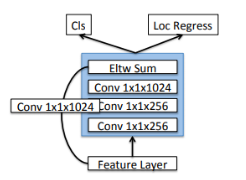
\includegraphics[width=0.5\textwidth]{predmod}
    \caption{Prediction Module}
    \label{fig:predmod1}
\end{figure}

\begin{figure}
    \centering
    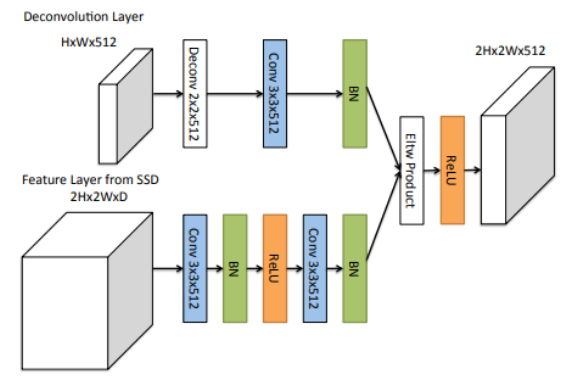
\includegraphics[width=0.75\textwidth]{deconvmod}
    \caption{Deconvolution Module}
    \label{fig:deconvmod1}
\end{figure}
\end{document}